\documentclass[12pt]{article} % Định dạng tài liệu, kích thước chữ 12pt

\usepackage{polyglossia} % Quản lí ngôn ngữ
\setdefaultlanguage{vietnamese}
\setotherlanguages{english}
\usepackage{fontspec} % Cung cấp khả năng sử dụng phông chữ OpenType và TrueType
\usepackage{
    amsmath, % Các lệnh toán học
    amsfonts, % Các kí hiệu toán học
    amssymb, % Các kí hiệu toán học
    amsthm % Môi trường định lí
}
\usepackage{unicode-math} % Cung cấp hỗ trợ cho các phông chữ toán học Unicode
\setmainfont{STIX Two Text} % Thiết lập phông chữ chính là STIX Two Text
\setmathfont{STIX Two Math} % Thiết lập phông chữ toán học là STIX Two Math

% \usepackage{ntheorem}

\usepackage[a4paper, left=2cm, right=2cm, top=2cm, bottom=2cm]{geometry} % Định dạng kích thước và lề trang

\usepackage{graphicx} % Hỗ trợ chèn hình ảnh vào tài liệu

\usepackage{xcolor} % Gói màu sắc để tùy chỉnh màu sắc

\usepackage[vietnamese]{hyperref} % Tạo liên kết và tham chiếu trong tài liệu
\hypersetup{
    colorlinks=true, % Kích hoạt màu sắc cho các liên kết
    linkcolor=blue, % Màu của liên kết nội bộ
    citecolor=blue, % Màu của liên kết tham chiếu
    filecolor=blue, % Màu của liên kết tập tin
    urlcolor=blue % Màu của liên kết URL
}
\renewcommand{\sectionautorefname}{Mục} % Đổi tên tự động của các liên kết phần mục từ "Section" thành "Mục"

\usepackage{bookmark} % Tạo mục lục nhanh và chính xác hơn

\usepackage[backend=biber,style=authoryear,sorting=none]{biblatex} % Quản lí tài liệu tham khảo với biblatex và biber
\addbibresource{references.bib} % Thêm tài liệu tham khảo từ tệp references.bib
\DeclareLanguageMapping{vietnamese}{vietnamese-english} % Định nghĩa ánh xạ ngôn ngữ cho tiếng Việt
\DeclareLanguageMapping{english}{english} % Định nghĩa ánh xạ ngôn ngữ cho tiếng Anh

\newcounter{myproblem} % Tạo một bộ đếm mới cho môi trường myproblem
\newenvironment{myproblem}[1][]{%
    \vspace{10pt} % Khảng cách từ trên xuống
    \noindent\textsc{Bài tập #1} % Định dạng tiêu đề môi trường myproblem
    \noindent
}{%
    \par
    \vspace{10pt} % Khoảng cách từ dưới lên
}
\newenvironment{mydotproblem}[1][]{%
    \vspace{10pt}
    \noindent\textsc{Bài tập. #1}
    \noindent
}{%
    \par
    \vspace{10pt} 
}
\newenvironment{mynumproblem}[1][]{%
    \refstepcounter{myproblem}
    \vspace{10pt}
    \noindent\textsc{Bài tập \theproblem. #1}
    \noindent
}{%
    \par
    \vspace{10pt} 
}

\newtheorem{theorem}{Định lí} % Thiết lập môi trường định lí, dựa trên gói amsthm

\title{Qui nạp tiến lùi}
% \author{Nguyễn Tấn Nhựt}
\date{}

\allowdisplaybreaks % Cho phép ngắt dòng trong các công thức toán học dài

\begin{document}

\maketitle
% \tableofcontents
% ----------------------------------------

% TÓM TẮT
\begin{abstract}
    Đôi khi phép qui nạp toán học thông thường chỉ diễn ra suôn sẻ đối với một vài tập con vô hạn thay vì toàn bộ số tự nhiên như mong muốn. Song song với đó là suy luận ngược mang lại thuận lợi hơn, nghĩa là đúng với \(n\) thì cũng đúng đối với \(n-1\). Nếu chỉ được thực hiện riêng lẻ, cái trước để lại nhiều khoảng trống, cái sau luôn dừng lại tại một giá trị \(n\) cố định được lấy làm cơ sơ qui nạp. Nhưng, nếu kết hợp lại cùng nhau, hai bước đó sẽ tạo thành một kiểu qui nạp hiệu quả để giải quyết một lớp vấn đề chuyên biệt, tạm gọi là giải được bằng qui nạp tiến lùi, trước tiến sau lùi. 
\end{abstract}
% ----------------------------------------

% MỤC 1
\section{Dẫn nhập}
Tổng các số tự nhiên liên tiếp \(1,2,\dots,n\) thường được tính nhanh bởi công thức
\[1+2+\cdots+n=\frac{n(n+1)}{2}.\]
Công thức nổi tiếng này có thể được chứng minh bằng lập luận qui nạp. Lập luận ấy như sau. Dễ thấy rằng nếu \(n=1\), công thức hiển nhiên đúng. Bây giờ giả sử rằng công thức đúng. Khi đó, 
\begin{align*}
    1+2+\cdots+n+(n+1)=\frac{n(n+1)}{2}+(n+1)=\frac{(n+1)(n+2)}{2}.
\end{align*}
Điều này nói lên rằng nếu công thức đúng với \(n\) thì cũng đúng với \(n+1\). Như vậy, công thức đã đúng với \(n=1\) nên nó đúng với \(n=2\), nó đã đúng với \(n=2\) nên nó đúng với \(n=3\), và cứ tiếp tục mãi. Vậy từ bây giờ ta đã có thể cùng công đó để tính tổng của bao nhiêu số tự nhiên liên tiếp tùy thích.

Qua phép chứng minh trên, phương pháp qui nạp chẳng những mạnh mẽ, mà nó còn giúp chúng ta một lập luận vững chắc để vượt qua khoảng trống mà cái vô hạn tạo ra thử thách chúng ta.

Trung bình số học của \(n\) số nguyên không âm \(x_1\), \(x_2\), \dots, \(x_n\) được định nghĩa là
\[\frac{x_1+x_2+\cdots+x_n}{n}\]
và trung bình hình học của chúng là
\[\sqrt[n]{x_1\cdot x_2\cdot\cdots\cdot x_n}.\]

\begin{theorem}
    Trung bình hình học của \(n\) số nguyên không âm \(x_1, x_2,\dots,x_n\) không vượt quá trung bình số học của chúng, nghĩa là
    \begin{equation}
        \sqrt[n]{x_1\cdot x_2\cdot\cdots\cdot x_n} \leq \frac{x_1+x_2+\cdots+x_n}{n} \label{eq:am-gm}
    \end{equation}
\end{theorem}
Bất đẳng thức này được gọi là bất đẳng thức của trung bình số học và trung bình hình học, hay ngắn gọn là bất đẳng thức AM-GM. Không quá xét nét, có thể xem phép chứng minh trình bày ngay đây là của Cố-xì, nó được tìm thấy trong Cours d'Analyse de l'École Royale Polytechique (trang 457). Thuật ngữ bất đẳng thức Cố-xì phải chăng bắt nguồn từ đây?

Thuật ngữ này tiết lộ nguyên lí hoạt động của phương pháp, bên cạnh đó, còn gọi là qui nạp Cố-xì\footnote{Cauchy}, cái tên gợi nhớ đến Augustin-Luois Cauchy, người phát minh ra nó trong phép chứng minh bất đẳng thức trung bình số học trung bình hình học\footnote{Bất đẳng thức AM-GM} theo cách riêng của mình.
% ----------------------------------------

% MỤC 2
\section{Chứng minh của Cố-xì} \label{sec:chung-minh-cua-co-si}
Trước tiên, viết lại trung bình hình học dưới dạng lũy thừa, bất đẳng thức \eqref{eq:am-gm} trở thành 
\[(x_1\cdot x_2\cdot\cdots\cdot x_n)^\frac{1}{n}\leq\frac{x_1+x_2+\cdots+x_n}{n},\]
và tương đương với 
\begin{equation}
    x_1\cdot x_2\cdot\cdots\cdot x_n\leq\left(\frac{x_1+x_2+\cdots+x_n}{n}\right)^n \label{eq:am-gm-dang-luy-thua}
\end{equation}
Chứng minh của Cố-xì được chia thành hai phân đoạn. Ở phân đoạn đầu, chứng minh cho các giá trị \(n\) là lũy thừa của \(2\), cụ thể là \(2,4,8,16,32\), v. v.. Ở phân đoạn cuối, cho các giá trị \(n\) còn lại, không là lũy thừa của \(2\). Như vậy, sau hai phân đoạn, bất đẳng thức đã được xác nhận với toàn bộ số tự nhiên. Lưu ý, \(n=1\) là trường hợ tầm thường và nếu các số hạng bằng nhau thì có đẳng thức.

Trường hợp đơn giản nhất mà không tầm thường là \(n=2\), khi đó
\begin{equation}
    x_1\cdot x_2 \leq \left(\frac{x_1+x_2}{2}\right)^2.
\end{equation}
Nó được rút ra từ
\begin{align*}
    x_1\cdot x_2&=\left(\frac{x_1+x_2}{2}\right)^2-\left(\frac{x_1-x_2}{2}\right)^2\\&\leq \left(\frac{x_1+x_2}{2}\right)^2.
\end{align*}
Lấy cái trước suy ra cái sau, làm tuần tự với \(n=4\), \(n=8\),\dots, \(n=2^m\), trong đó \(m\) nguyên dương và lớn hơn \(3\), sẽ có
\begin{align*}
    x_1x_2x_3x_4&=(x_1x_2)(x_3x_4)\\&\leq\left(\frac{x_1+x_2}{2}\right)^2\left(\frac{x_3+x_4}{2}\right)^2\\&=\left(\frac{x_1+x_2}{2}\cdot\frac{x_3+x_4}{2}\right)^2\\&\leq\left(\left(\frac{\frac{x_1+x_2}{2}+\frac{x_3+x_4}{2}}{2}\right)^2\right)^2\\&=\left(\frac{x_1+x_2+x_3+x_4}{4}\right)^4,
\end{align*}
\begin{align*}
    x_1x_2x_3x_4x_5x_6x_7x_8&=(x_1x_2x_3x_4)(x_5x_6x_7x_8)\\&\leq\left(\frac{x_1+x_2+x_3+x_4}{4}\right)^4\left(\frac{x_5+x_6+x_7+x_8}{4}\right)^4\\&=\left(\frac{x_1+x_2+x_3+x_4}{4}\cdot\frac{x_5+x_6+x_7+x_8}{4}\right)^4\\&\leq\left(\left(\frac{\frac{x_1+x_2+x_3+x_4}{4}+\frac{x_5+x_6+x_7+x_8}{4}}{2}\right)^2\right)^4\\&=\left(\frac{x_1+x_2+x_3+x_4+x_5+x_6+x_7+x_8}{8}\right)^8,\dots,
\end{align*}
\begin{align}
    x_1x_2\cdots x_{2^m}\leq\left(\frac{x_1+x_2+\cdots+x_{2^m}}{2^m}\right)^{2^m}. \label{eq:am-gm-2-mu-m}
\end{align}
\begin{figure}[htbp]
    \centering
    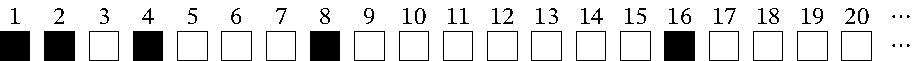
\includegraphics{./tex-images/cac-so-tu-nhien-2-mu/cac-so-tu-nhien-2-mu.pdf}
    \caption{Ô đen đại diện cho các số tự nhiên đã được xác nhận tới thời điểm này. Việc tiếp theo là tìm cách tô đen các ô còn lại.}
\end{figure}
Khi \(n\) không phải một trong các giá trị \(2,4,8,16,\dots\) và giả sử rằng \(n<2^m\), áp dụng \eqref{eq:am-gm-2-mu-m} với \(2^m-n\) số hạng cuối đều là \(\frac{x_1+x_2+\cdots+x_n}{n}\), cho kết Quản
\begin{align*}
    x_1x_2\cdots x_n\left(\frac{x_1+x_2+\cdots+x_n}{n}\right)^{2^m-n}\\&\leq\left(\frac{x_1+x_2+\cdots+x_n+(2^n-m)\frac{x_1+x_2+\cdots+x_n}{n}}{2^m}\right)\\&=\left(\frac{x_1+x_2+\cdots+x_n}{n}\right)^{2^m}
\end{align*}
Từ đây, suy ra
\[x_1x_2\cdots x_n\leq\left(\frac{x_1+x_2+\cdots+x_n}{n}\right)^n.\]
Điều này khẳng định đúng với \(2^m\) cũng đúng với tất cả các giá trị nguyên dương bé hơn.
% ----------------------------------------

% MỤC 3
\section{Qui nạp tiến lùi}
Kí hiệu ngắn gọn cho bất đẳng thức \eqref{eq:am-gm} là \(P(n)\). Dựa trên phương pháp qui nạp toán học thông thường, và có thêm vào một số thuật ngữ, qui trình chứng minh của Cố-xì ở \autoref{sec:chung-minh-cua-co-si} có thể hình thức hóa thành ba bước như dưới đây.
\begin{itemize}
    \item Cơ sở, chứng minh \(P(2)\).
    \item Qui nạp tiến, chứng minh \(P(2^n)\) kéo theo \(P(2^{n+1})\).
    \item Qui nạp lùi, chứng minh \(P(2^n)\) kéo theo \(P(m)\), với mọi \(m<2^n\).
\end{itemize}
Hãy tinh tế nhận định rằng hai bước đầu đã tạo ra một cơ sở vô hạn phần tử, thay vì một cơ sở chỉ có duy nhất phần tử như qui nạp thông thường, đáp ứng cho qui nạp lùi ở bước cuối. Cách nhìn này mang lại một quan niệm
% ----------------------------------------

% BÀI TẬP
\begin{myproblem}
\begin{enumerate}
    \item Hãy biện luận theo qui trình bên dưới để chứng minh bất đẳng thức AM-GM.
    \begin{itemize}
        \item Chứng minh \(P(2)\).
        \item Chứng minh \(P(n)\) kéo theo \(P(2n)\).
        \item Chứng minh \(P(n)\) kéo theo \(P(n-1)\).
    \end{itemize}
    \item Cho \(n\) là một số nguyên dương và \(x_1,x_2,\dots,x_n\) là các số thuộc khoảng \(\left(0,\frac{1}{2}\right)\). Theo Ky Fan, 
    \begin{align*}
        \frac{x_1x_2\cdots x_n}{(x_1+x_2+\cdots+x_n)^n}\leq\frac{(1-x_1)(1-x_2)\cdots(1-x_n)}{(1-x_1)+(1-x_2)+\cdots+(1-x_n)}.
    \end{align*}
    Hãy dùng qui nạp tiến lùi chứng minh bất đẳng thức Ky Fan.

    Gợi ý. Khi \(n=2\) nó tương đương với điều hiển nhiên \(x_1+x_2\leq 1\) theo giả thiết. Nhằm dễ qui nạp hơn, hãy đưa về dạng tương đương 
    \begin{align*}
        \left(\frac{n}{x_1+x_2+\cdots+x_n}-1\right)^n\leq\left(\frac{1}{x_1}-1\right)\left(\frac{1}{x_2}-1\right)\cdots\left(\frac{1}{x_n}-1\right).
    \end{align*}
\end{enumerate}
\end{myproblem}
% ----------------------------------------
\cite{BradleySandifer2009}
% THƯ MỤC
\printbibliography

\end{document}
